%
% Main document
% ===========================================================================
% This is part of the document "Project documentation template".
% Authors: aescd5,knece1
%

%---------------------------------------------------------------------------
\documentclass[
	a4paper,					% paper format
	10pt,
	french,		% fontsize
	%twoside,					% double-sided
	%openright,				% begin new chapter on right side
	notitlepage,			% use no standard title page
	parskip=half,			% set paragraph skip to half of a line
]{scrreprt}					% KOMA-script report
%---------------------------------------------------------------------------

\raggedbottom
\KOMAoptions{cleardoublepage=plain}			% Add header and footer on blank pages


% Load Standard Packages:
%---------------------------------------------------------------------------
\usepackage[standard-baselineskips]{cmbright}

\usepackage{babel}										% german hyphenation
%\usepackage[latin1]{inputenc}  							% Unix/Linux - load extended character set (ISO 8859-1)
\usepackage[utf8]{inputenc}  							% Windows - load extended character set (ISO 8859-1)
\usepackage[T1]{fontenc}											% hyphenation of words with ä,ö and ü
\usepackage{textcomp}													% additional symbols
\usepackage{ae}																% better resolution of Type1-Fonts 
\usepackage{fancyhdr}													% simple manipulation of header and footer 
\usepackage{etoolbox}													% color manipulation of header and footer
\usepackage{graphicx}                      		% integration of images
\usepackage{float}														% floating objects
\usepackage{caption}													% for captions of figures and tables
\usepackage{booktabs}													% package for nicer tables
\usepackage{tocvsec2}													% provides means of controlling the sectional numbering
\usepackage{listings}
\usepackage{natbib}   % omit 'round' option if you prefer square brackets
\bibliographystyle{abbrvnat}
\setcitestyle{authoryear,open={(},close={)}}
%---------------------------------------------------------------------------

% Load Math Packages
%---------------------------------------------------------------------------
\usepackage{amsmath}                    	   	% various features to facilitate writing math formulas
\usepackage{amsthm}                       	 	% enhanced version of latex's newtheorem
\usepackage{amsfonts}                      		% set of miscellaneous TeX fonts that augment the standard CM
\usepackage{amssymb}													% mathematical special characters
\usepackage{exscale}													% mathematical size corresponds to textsize
%---------------------------------------------------------------------------

% Custom commands
%---------------------------------------------------------------------------
%\newcommand{\CC}{C\nolinebreak\hspace{-.05em}\raisebox{.4ex}{\tiny\bf +}\nolinebreak\hspace{-.10em}\raisebox{.4ex}{\tiny\bf +}}

%\newcommand{\CS}{C\nolinebreak\hspace{-.05em}\raisebox{.6ex}{\scriptsize\bf \#}}
%---------------------------------------------------------------------------

% Package to facilitate placement of boxes at absolute positions
%---------------------------------------------------------------------------
\usepackage[absolute]{textpos}
\setlength{\TPHorizModule}{1mm}
\setlength{\TPVertModule}{1mm}
%---------------------------------------------------------------------------					
			
% Definition of Colors
%---------------------------------------------------------------------------
\RequirePackage{color}                          % Color (not xcolor!)
\definecolor{linkblue}{rgb}{0,0,0.8}            % Standard
\definecolor{darkblue}{rgb}{0,0.08,0.45}        % Dark blue
\definecolor{bfhgrey}{rgb}{0.41,0.49,0.57}      % BFH grey
%\definecolor{linkcolor}{rgb}{0,0,0.8}     			% Blue for the web- and cd-version!
\definecolor{linkcolor}{rgb}{0,0,0}        			% Black for the print-version!
%---------------------------------------------------------------------------

% Hyperref Package (Create links in a pdf)
%---------------------------------------------------------------------------
\usepackage[
	pdftex,ngerman,bookmarks,plainpages=false,pdfpagelabels,
	backref = {false},										% No index backreference
	colorlinks = {true},                  % Color links in a PDF
	hypertexnames = {true},               % no failures "same page(i)"
	bookmarksopen = {true},               % opens the bar on the left side
	bookmarksopenlevel = {0},             % depth of opened bookmarks
	pdftitle = {Template für Bachelor Thesis},	   	% PDF-property
	pdfauthor = {brd3},        					  % PDF-property
	pdfsubject = {LaTeX Template},        % PDF-property
	linkcolor = {linkcolor},              % Color of Links
	citecolor = {linkcolor},              % Color of Cite-Links
	urlcolor = {linkcolor},               % Color of URLs
]{hyperref}
%---------------------------------------------------------------------------

% Set up page dimension
%---------------------------------------------------------------------------
\usepackage{geometry}
\geometry{
	a4paper,
	left=28mm,
	right=15mm,
	top=30mm,
	headheight=20mm,
	headsep=10mm,
	textheight=242mm,
	footskip=15mm
}
%---------------------------------------------------------------------------

% Makeindex Package
%---------------------------------------------------------------------------
%\usepackage{makeidx}                         		% To produce index
%\makeindex                                    	% Index-Initialisation
%---------------------------------------------------------------------------
% Glossary Package
%---------------------------------------------------------------------------
% the glossaries package uses makeindex
% if you use TeXnicCenter do the following steps:
%  - Goto "Ausgabeprofile definieren" (ctrl + F7)
%  - Select the profile "LaTeX => PDF"
%  - Add in register "Nachbearbeitung" a new "Postprozessoren" point named Glossar
%  - Select makeindex.exe in the field "Anwendung" ( ..\MiKTeX x.x\miktex\bin\makeindex.exe )
%  - Add this [ -s "%tm.ist" -t "%tm.glg" -o "%tm.gls" "%tm.glo" ] in the field "Argumente"
%
% for futher informations go to http://ewus.de/tipp-1029.html
%---------------------------------------------------------------------------
%\usepackage[nonumberlist]{glossaries}
%\makeglossaries
%
\newglossaryentry{BibTeX}{name={BibTeX},description={Programm zur Erstellung von Literaturangaben und -verzeichnissen in \TeX- oder \LaTeX-Dokumenten}}
\newglossaryentry{StwVrz}{name={Stichwortverzeichnis},description={Verzeichnis mit Stichworten aus dem Text}}



%---------------------------------------------------------------------------

% Intro:
%---------------------------------------------------------------------------
\begin{document}                              	% Start Document
\settocdepth{section}														% Set depth of toc
\pagenumbering{roman}														
%---------------------------------------------------------------------------

\providecommand{\titel}{Intégration continues}					% Titel der Arbeit aus Datei titel.tex lesen
\providecommand{\versionnumber}{1.2}			%  Hier die aktuelle Versionsnummer eingeben
\providecommand{\versiondate}{01.02.2014}		%  Hier das Datum der aktuellen Version eingeben				% Versionsnummer und -datum aus Datei version.tex lesen

% Set up header and footer
%---------------------------------------------------------------------------
\makeatletter
\patchcmd{\@fancyhead}{\rlap}{\color{bfhgrey}\rlap}{}{}		% new color of header
\patchcmd{\@fancyfoot}{\rlap}{\color{bfhgrey}\rlap}{}{}		% new color of footer
\makeatother

\fancyhf{}																		% clean all fields
\fancypagestyle{plain}{												% new definition of plain style	
	\fancyfoot[OR,EL]{\footnotesize \thepage} 	% footer right part --> page number
	\fancyfoot[OL,ER]{\footnotesize \titel, Version \versionnumber, \versiondate}	% footer even page left part 
}

\renewcommand{\chaptermark}[1]{\markboth{\thechapter.  #1}{}}
\renewcommand{\headrulewidth}{0pt}				% no header stripline
\renewcommand{\footrulewidth}{0pt} 				% no bottom stripline

\pagestyle{plain}
%---------------------------------------------------------------------------


% Title Page and Abstract
%---------------------------------------------------------------------------
%%
% Project documentation template
% ===========================================================================
% This is part of the document "Project documentation template".
% Authors: brd3, kaa1
%

\begin{titlepage}


% BFH-Logo absolute placed at (28,12) on A4 
% Actually not a realy satisfactory solution but working.
%---------------------------------------------------------------------------
\setlength{\unitlength}{1mm}
\begin{textblock}{20}[0,0](28,12)
	
\includegraphics[scale=1.0]{bilder/BFH_Logo_B.png}
\end{textblock}
\color{black}

% Institution / Titel / Untertitel / Autoren / Experten:
%---------------------------------------------------------------------------
\begin{flushleft}

\vspace*{21mm}

\fontsize{26pt}{40pt}\selectfont 
\titel 				\\							% Titel aus der Datei vorspann/titel.tex lesen
\vspace{2mm}

\fontsize{16pt}{24pt}\selectfont\vspace{0.3em}
Hier steht ein Untertitel 			\\							% Untertitel eingeben
\vspace{5mm}

\fontsize{10pt}{12pt}\selectfont
\textbf{Art der Arbeit (Semesterarbeit / Bachelorthesis / etc.)} \\									% eingeben
\vspace{7mm}

% Abstract (eingeben):
%---------------------------------------------------------------------------
\begin{textblock}{150}(28,100)
\fontsize{10pt}{12pt}\selectfont
[Kurztext (Abstract) einf�gen, falls gew�nscht] \\ 
Dieses Dokument dient als Vorlage f�r die Erstellung von Berichten nach den Richtlinien der BFH. Die Vorlage ist in \LaTeX{} erstellt und unterst�tzt das automatische Erstellen von diversen Verzeichnissen, Literaturangaben, Indexierung und Glossaren. Dieser kleine Text ist eine Zusammenfassung �ber das vorliegenden Dokument mit einer L�nge von 4 bis max. 8 Zeilen. \\
Das Titelbild kann in den Zeilen 157/158 der Datei template.tex ein- oder ausgeschaltet werden.
\end{textblock}

\begin{textblock}{150}(28,225)
\fontsize{10pt}{17pt}\selectfont
\begin{tabbing}
xxxxxxxxxxxxxxx\=xxxxxxxxxxxxxxxxxxxxxxxxxxxxxxxxxxxxxxxxxxxxxxx \kill
Studiengang:	\> [z.B. Elektro- und Kommunikationstechnik]	\\			% Namen eingeben
Autoren:		\> [Test Peter, M�ster R�s�]		\\					% Namen eingeben
Betreuer:	\> [Dr.~Xxxx Xxxx, Dr.~Yyyy Yyyy]		\\					% Namen eingeben
Auftraggeber:	\> [Wwwww AG]						\\					% Namen eingeben
Experten:		\> [Dr.~Zzzz Zzzz]				\\					% Namen eingeben
Datum:			\> \versiondate					\\		% aus Datei vorspann/version.tex lesen
\end{tabbing}

\end{textblock}
\end{flushleft}

\begin{textblock}{150}(28,280)
\noindent 
\color{bfhgrey}\fontsize{9pt}{10pt}\selectfont
Berner Fachhochschule | Haute �cole sp�cialis�e bernoise | Bern University of Applied Sciences
\color{black}\selectfont
\end{textblock}


\end{titlepage}

%
% ===========================================================================
% EOF
%
		% activate for Titelseite ohne Bild
%
% Project documentation template
% ===========================================================================
% This is part of the document "Project documentation template".
% Authors: brd3, kaa1
%

\begin{titlepage}


% BFH-Logo absolute placed at (28,12) on A4 and picture (16:9 or 15cm x 8.5cm)
% Actually not a realy satisfactory solution but working.
%---------------------------------------------------------------------------
\setlength{\unitlength}{1mm}
\begin{textblock}{20}[0,0](28,12)
	
\includegraphics[scale=1.0]{bilder/BFH_Logo_B.png}
\end{textblock}

\begin{textblock}{154}(28,48)
	\begin{picture}(150,2)
		\put(0,0){\color{bfhgrey}\rule{150mm}{2mm}}
	\end{picture}
\end{textblock}

\begin{textblock}{154}[0,0](28,50)
	
\includegraphics[scale=0.6]{bilder/CI_titleImage.png}			% Titelbild definieren
\end{textblock}

\begin{textblock}{154}(28,135)
	\begin{picture}(150,2)
		\put(0,0){\color{bfhgrey}\rule{150mm}{2mm}}
	\end{picture}
\end{textblock}
\color{black}

% Institution / Titel / Untertitel / Autoren / Experten:
%---------------------------------------------------------------------------
\begin{flushleft}

\vspace*{115mm}

\fontsize{26pt}{28pt}\selectfont 
\titel 				\\							% Titel aus der Datei vorspann/titel.tex lesen
\vspace{2mm}

\fontsize{10pt}{12pt}\selectfont
\textbf{Rapport 2 - Séminaire Info 2016} \\									% eingeben
\vspace{3mm}

\begin{textblock}{150}(28,225)
\fontsize{10pt}{17pt}\selectfont
\begin{tabbing}
xxxxxxxxxxxxxxx\=xxxxxxxxxxxxxxxxxxxxxxxxxxxxxxxxxxxxxxxxxxxxxxx \kill
Filière d'études:	\> Informatique	\\			% Namen eingeben
Auteurs:		\> Emanuel Knecht, David Aeschlimann		\\					% Namen eingeben
Conseiller:	\> 		Dr. Bernhard Anrig		\\					% Namen eingeben
Date:			\> \versiondate					\\		% aus Datei vorspann/version.tex lesen
\end{tabbing}

\end{textblock}
\end{flushleft}

\begin{textblock}{150}(28,280)
\noindent 
\color{bfhgrey}\fontsize{9pt}{10pt}\selectfont
Berner Fachhochschule | Haute école spécialisée bernoise | Bern University of Applied Sciences
\color{black}\selectfont
\end{textblock}


\end{titlepage}

%
% ===========================================================================
% EOF
%
			% activate for Titelseite mit Bild
%---------------------------------------------------------------------------

% Table of contents
%---------------------------------------------------------------------------
\tableofcontents
%\cleardoublepage
%---------------------------------------------------------------------------

% Main part:
%---------------------------------------------------------------------------
\pagenumbering{arabic}

\chapter{Einleitung}
\label{chap:einleitung}

Dieses Dokument ist der schriftliche Teil des Informatikseminars an der Berner Fachhochschule. In den kommenden Kapiteln wird die Aspektorientierte Programmierung mit AspectJ vorgestellt und erkl�rt.

\nocite{laddad:aspectj}

\section{Auftrag}
\label{sec:einleitung_auftrag}



\section{Vorgehen}
\label{sec:einleitung_vorgehen}


\chapter{Intégration Continue}
\label{chap:integrationcontinue}

\section{Histoire}
La notion \textit{Intégration Continue} était mentionné dans un livre de Grady Booch en 1994 pour la première foi\footnote{\cite{boochooad}}. Il parlait d'une intégration continue par des publications interne et chaque publication apporte l'application plus proche à la version finale.

La prochaine foi que l'intégration continue était sous les feux de l'actualité était avec la publication des concepts de \textit{Extreme Programming} en forme d'un livre en 1999.
Là inclue est l'idée d'avoir une machine dédié à l'intégration du code et les pairs de développeurs réunissant, intégrant et testant le code source après chaque changement.\footnote{\cite{robertshistory}}

Une autre personne qui a gravé la notion \textit{Intégration Continue} est Martin Fowler. Il a publié un article sur le sujet en 2000 et révisé celui-ci six ans plus tard.\footnote{\cite{fowlerci}} Dans cet article il essayerait de donner une définition de l'IC et des meilleures pratiques. Martin Fowler travaillait chez ThoughtWorks, l'entreprise responsable pour la publication du première serveur d'\textit{Intégration Continue} "Cruise Control". Il est souvent cité comme personne-clé si on parle de l'IC.

Le premier livre publié sur la matière était "Continous Integration"\footnote{\cite{duvallconint}} en 2007. Naturellement il y a beaucoup d'autre livres traitant des technologie ou outils concrètes. Aujourd'hui le plus part d'entreprises implémentes quelques ou tous les aspects de l'IC.

\nocite{wikici}
\newpage

\section{Aperçu}
Pour pouvoir comprendre le concept de base de l'intégration continue il est nécessaire de connaitre le processus de développement logiciel ordinaire. L'intégration Continue n'exige pas de méthode de gestion de projets spécifique, mais est souvent utilisé avec des approches agiles, car elle les complètent parfaitement. Voici un diagramme d'un processus pareil. \footnote{Source http://www.techtipsnapps.com/2015/04/most-successful-software-development.html}

\begin{figure}[H]
	\centering
		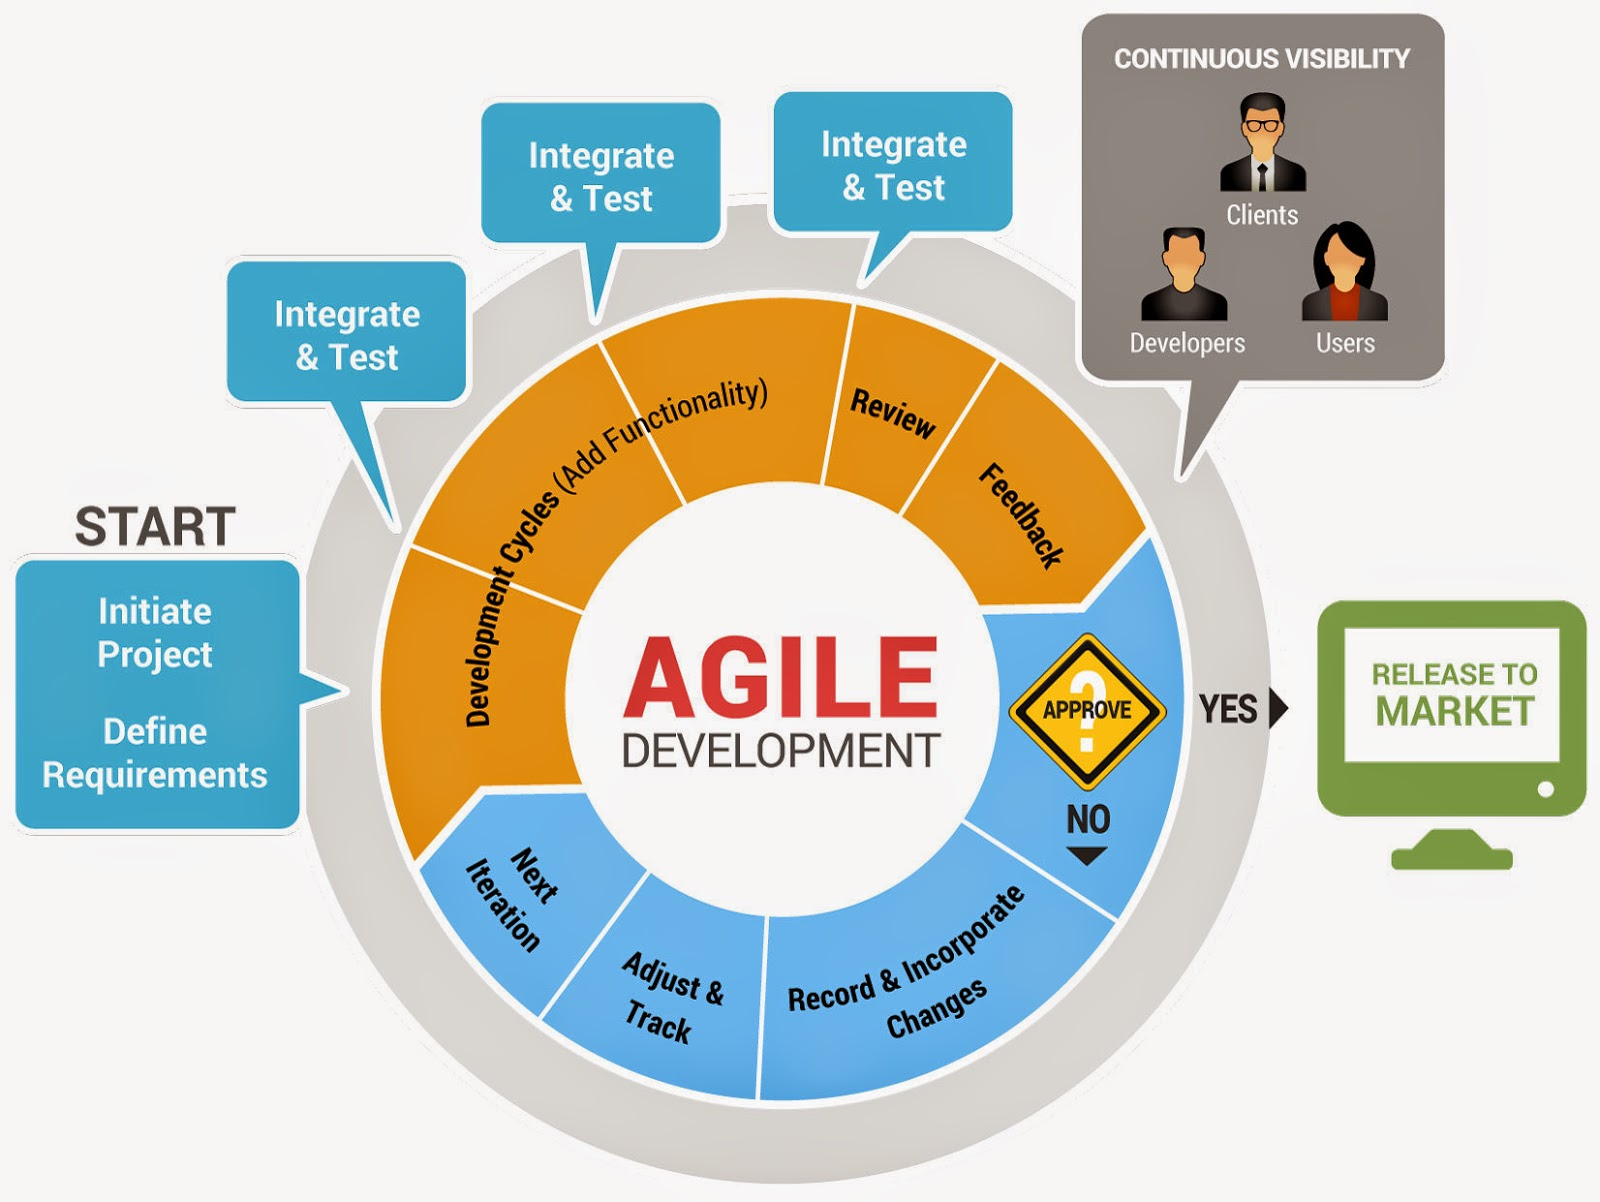
\includegraphics[scale=0.25]{bilder/agile_methodology}
	\caption{Processus de développement logiciel}
	\label{fig:processus}
\end{figure}

Les étapes récurrent sont le développement, les testes, les contrôles, le déploiement, la réaction du client et après ça une nouvelle itération. L'idée principale de L'IC est d'automatiser des devoirs des développeurs ou d'offrir des aides pendants tous ces étapes du processus de développement.
Pendant presque tous les projets de développement on travaille en équipe. Tous les développeurs font des changements et ajoutent de la fonctionnalité chaque jour. C'est pour cela qu'il est nécessaire de réunir ces changements régulièrement et de vérifier si tous les composants marche et coopère comme voulu (testes).\\\\
Ce processus de réunification s'appelle l'intégration. Si l'intégration est faite continuellement on parle de l'\textbf{Intégration Continue}. Mais une Intégration Continue à la lettre, chaque minute ou même en temps réel, n'est pas faisable ou aidant. C'est pour ça qu'une intégration exécuter au moins une foi par jour est normalement considéré suffisante, naturellement le plus souvent le mieux.\\
De plus cette intégration doit être facile et automatisée, comme pousser un bouton. Après lancer le processus d'intégration tous le reste doit être contrôlé par le système IC. La définition et l'étendue de l'IC est ouverte, pas strictement limité et fortement dépendant de l'application à développer. Mais il y a quelques éléments qui apparaissent dans tous les systèmes d'IC.
\newpage

\subsection{Architecture exemplaire}
Voici une architecture normale en travaillant avec un système d'intégration continue.
\begin{figure}[H]
	\centering
		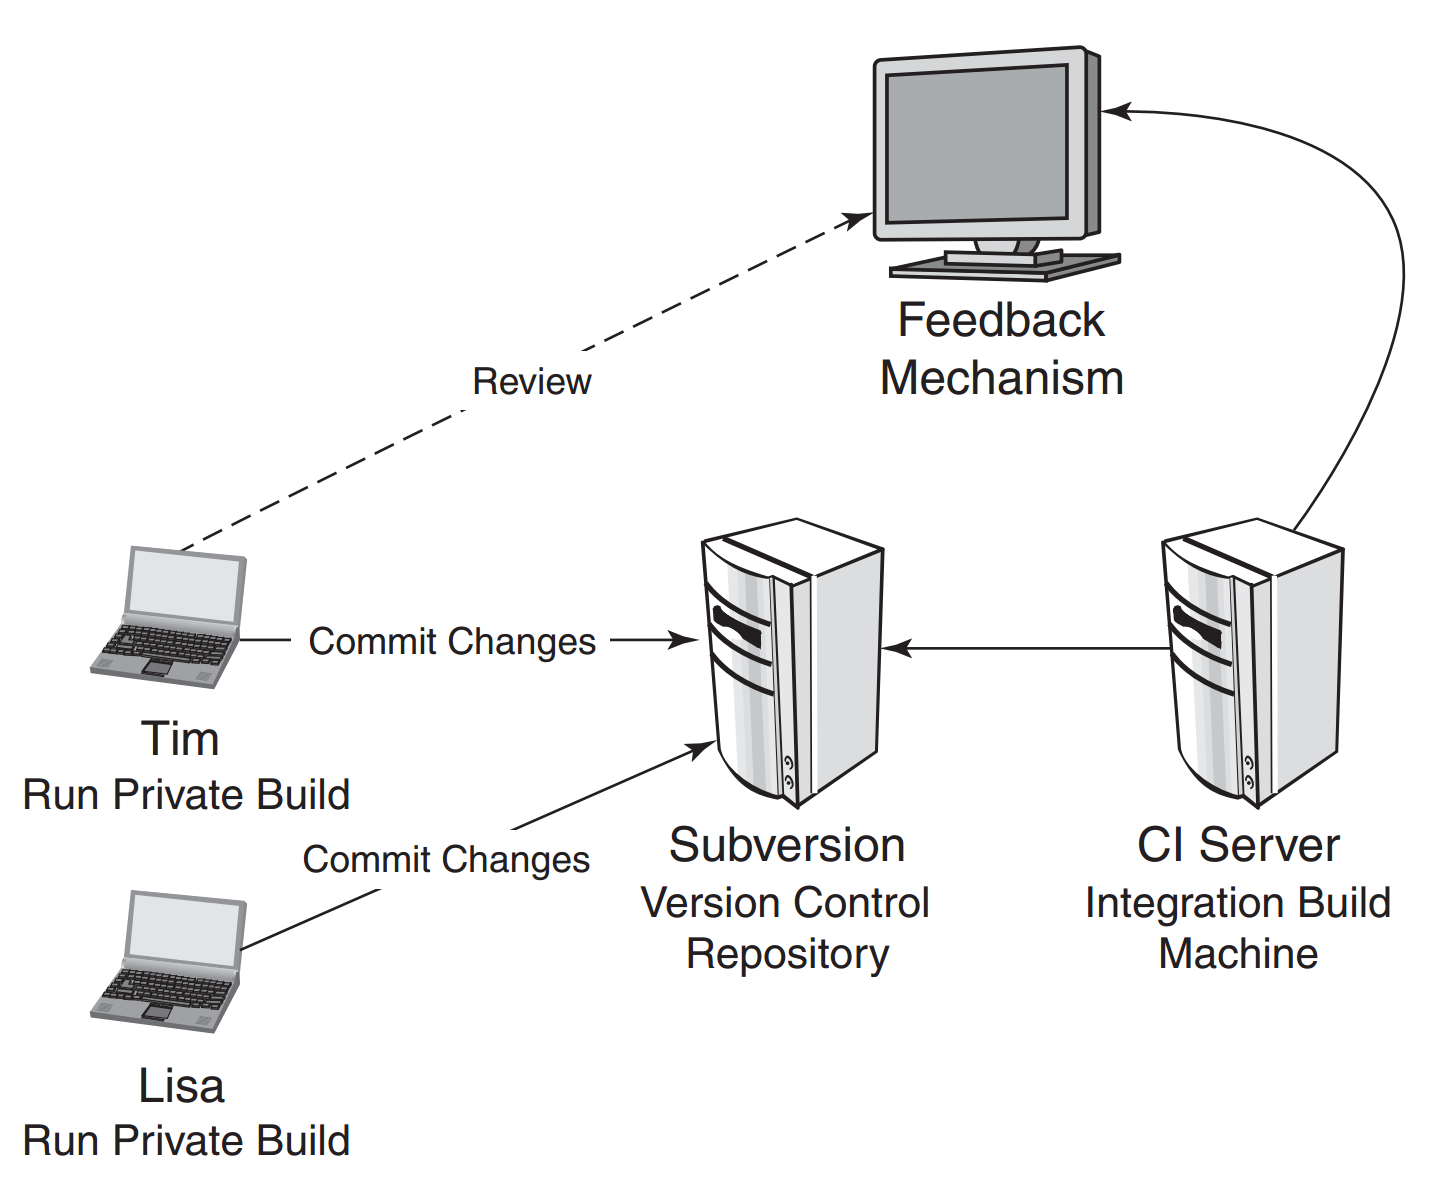
\includegraphics[scale=0.6]{bilder/architecture_exemplaire}
	\caption{Architecture exemplaire}
	\label{fig:processus}
\end{figure}

\textbf{Développement locale}\\
Tous les développeurs travaillent sur ses machines privées ou des machines de l'entreprise. Avant d'ajouter de la fonctionnalité la version la plus actuelle est téléchargé du dépôt centrale. Après changer le code il est nécessaire de faire une construction et d'exécuter les testes unitaires localement. Si tout fonctionne les changements sont commit sur le dépôt centrale.\\\\
\textbf{Dépôt centrale}\\
Le dépôt centrale est normalement un système de gestion de versions comme Subversion ou Git. Il est installé sur un serveur dédié. Tous les développeur reçoivent de l'accès pour commettre des changements là dessus. Ce faisant il est possible d'identifier qui a changé quoi en cas que quelque chose ne marche plus.\\\\
\textbf{Serveur de l'intégration Continue} \\
Le serveur de l'intégration Continue est la partie centrale du système. Il est aussi installé sur un serveur dédie, quelque foi sur la même machine que le dépôt centrale. Le serveur IC contrôle régulièrement s'il y a une nouvelle version dans le dépôt centrale. Si c'est le cas le serveur prends le code et démarre le processus d'intégration. Les étapes du processus doivent normalement être configurer une fois par projet. Quelques exemples pour des étapes possibles:
\begin{itemize}
\item Construction du code
\item Testes unitaires, testes d'intégration ou testes fonctionnelle
\item Inspections
\item Création de sous-système ou déploiement
\end{itemize}
Si on inclue le déploiement dans le processus d'intégration, il ne s'agit strictement plus de l'intégration Continue, mais aussi du \textbf{Déploiement et de la Livraison Continue} (Continous Deployment, Continuous Delivery). 
\\\\
\textbf{Information en retour}\\
Après finir ce processus d'intégration les résultats des étapes sont affiché sur un interface d'utilisateur centrale, souvent une page web. Pour toutes les étapes il est possible de configurer si l'échec de l'étape amène l'échec du processus complet. Si il y a des erreurs les développeurs et les personnes responsable peuvent être informer par des emails. Quelques entreprises installe des écrans dans les bureaux qui affichent les dernières résultats en temps réelle.\\
\section{Concepts de l'intégration Continue}

\subsection{Construction continue}
L'idée de la construction continue est de définir le processus de construction une foi, normalement dans un fichier de construction, qui est ensuite utilisé par le serveur d'IC de construire le projet à chaque intégration. Dans le fichier de construction les fichiers source et les dépendances sont définit. Tous les langages de programmations utilisent des outils de construction différents. Voici deux example.

\subsubsection{Java}
Ant (Another neat tool) a apparu 2000, le premier logiciel de construction pour Java.
Aujourd'hui Ant et ses produits de concurrence Maven(2002) et Gradle(2012) sont inévitable si on utilise Java.
Dans ce moment environ 70 \% des développeurs Java utilisent Maven, 15 \% Ant et 15\% Gradle. Le concept est pareille comme en C++. 
%EMAAA Quelle? VIDDY Ke ahnig me woni das uf em netz gfunde ha, weiss nur no das es veraltet isch gsi.. wahrschinlich isch gradle inzwüsche no höcher.. ha keni aktuelle statistike gfunde.. drum hani ja "environ" gschribe..
\subsubsection{C/C++}
Le premier logiciel de construction était make, qui existes depuis 1976 (Stuart Feldman, Bell Labs). Sur les plateformes basé sur Unix make est encore utilisé pour construire des exécutables.
Pour construire une application avec make if faut fournir un fichier makefile qui contiens les instructions de compilation. Supposant on a un logiciel avec les fichiers: \\ \\

\begin{tabular}{ll}
functions.h&squared.c\\
{\lstinputlisting[language=C]{../project/cpp_make_sample/functions.h}}&{\lstinputlisting[language=C,]{../project/cpp_make_sample/squared.c}}\\
\end{tabular}


factorial.c
\lstinputlisting[language=C]{../project/cpp_make_sample/factorial.c}


main.cpp
\lstinputlisting[language=C]{../project/cpp_make_sample/main.cpp}

La commande pour compiler ce projet manuellement est:
$$g++\;main.cpp\;squared.cpp\;factorial.cpp\;-o\;hello$$
Pour un projet si petit c'est assez simple, mais avec plus de fichiers ça devient déroulant très vite.
Par exemple si on a beaucoup de dépendances ou une application multi-plateforme c'est très difficile de ne pas oublier un élément.
\newpage
C'est pour ça qu'il existe l'option de créer des makefile. Le makefile liste tous les fichiers et dépendances du projet.
\lstinputlisting[language=make,caption={Makefile sans variables}]{../project/cpp_make_sample/Makefile1.}
Si on regarde le fichier Makefile correspondant, on voit que ça ne simplifie pas encore notre vie. Une prochaine étape est l'introduction des variables dans le makefile.
\lstinputlisting[language=make,caption={Makefile avec variables}]{../project/cpp_make_sample/Makefile2.}

Ce fichier est plus court et très adaptable, mais il n'est pas lisible.
En utilisant l'outil cmake on peut générer les fichiers Makefile automatiquement (et autres fichiers de projet comme ".sln").
Dans le fichier CMakeLists.txt on définit quels fichiers il faut compiler et quels sont les dépendances.
\lstinputlisting[language=make,caption={CMakeLists.txt}]{../project/cpp_make_sample/CMakeLists.txt}

Tous ses types de construction peuvent être automatiser avec un serveur d'IC.
\newpage

\subsection{Intégration continue de base de données}

Le plus part de logiciel utilisent une méthode pour persister des données, beaucoup de fois des bases de données. Le code source pour générer cette base de données doit être traiter comme tous le reste du code d'un projet. C'est nécessaire qu'il soit aussi commit sur le dépot centrale et qu'on teste et fait des inspections là dessus.

\subsubsection{Automatisation de l'intégration}
Si le code de la base de données est aussi mis sur le dépot centrale, le processus de l'intégration de base de données peut être automatisé. Ce processus peut devenir assez complexe avec différent environnements. Les serveurs, les noms d'utilisateur, les mots de passe ou bien les données de test ou de système peuvent différer pour chaque environnement.
\begin{figure}[H]
	\centering
		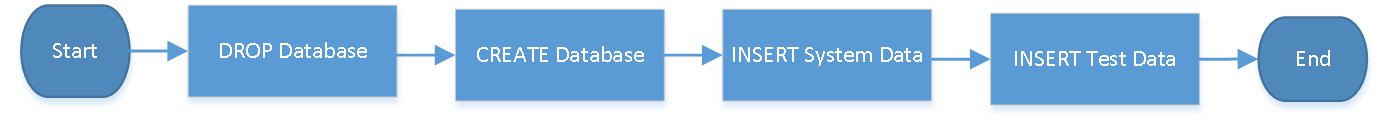
\includegraphics[scale=1]{bilder/database_integration}
	\caption{Processus de l'intégration de base de données}
	\label{fig:processus}
\end{figure}

C'est pour ça qu'une automatisation de ce processus est indispensable. Une automation est réalisé en insérant une section dans le script de construction uniquement pour les opérations de l'intégration de base de données. L'intervalle et l'étendue de l'exécution de ce processus sont pas les mêmes pour tous les projets. Pour quelques projets ça pourrait être trop lourds de recrée la base de données à chaque changement sur le dépôt centrale. Avec l'outil de construction Maven et le plugin "sql-maven-plugin" il est possible de définir quelle base de données est visé et quelles commandes sont exécuté. Voici une partie d'un tel script.\footnote{Pour l'exemple complète \cite{mvnsql}}

\lstinputlisting[language=XML]{./anhang/db_mvn_sql.xml}

\subsubsection{Instance de base de donnée locale}

Pour que cette approche fonctionne optimalement tous les développeurs doivent avoir l'autorisation de changer la définition de la base de données. Pour éviter des conflits pendant le développement tous les développeurs ont besoin d'une instance de cette base de données sur leur machines locales. Si on travaille avec une instance centrale à chaque changement il y a le danger de casser le code que quelqu'un d'autre est en train de développer.
\newpage


\subsection{Tests continue}
Les tests existes pour contrôler la fonctionnalité d'un bout de code, d'un système ou d'une application complète. Le premier principe de base pour des tests automatisés est "Fail fast" (Échouer vite). On distingue trois types de tests différents. Comme règle d'or on peut dire que les tests unitaires prend des secondes, les testes d'intégration prend des minutes et les tests d'acceptation prend des heures.\footnote{\citep{artofunittesting}}

\subsubsection{Tests unitaires}
Les tests unitaires vérifient le bon fonctionnement d'un bout de code. Pour les parties du code qui ne sont pas testable atomiquement on introduit des objets mock qui permettent des tests de fonctionnement vite et sans effets secondaires. 
\subsubsection{Tests d'intégration}
Après avoir tester les composant atomiquement, il est aussi nécessaire de tester l'interaction de ces composant avec des systèmes secondaire comme le système de fichier ou une base de données. Après ces tests d'intégration les erreurs logiques et d'intégration doivent être éliminé.
\subsubsection{Tests d'acceptation}
Les testes d'acceptation contrôle si les exigences du client sont respecté. \\
Il y a différents types de test d'acceptation:
\begin{enumerate}
 \item \textit{Tests d'interface utilisateur automatisé (code)}
 \\Pour ces tests il faut spécifier des scénario. Une programme teste accède l'application et exécute le scénario avec des interactions avec l'interface d'utilisateur.
 \item \textit{Tests de performance}
 \\Ces tests montrent quelles parties du code prennent la plupart des ressources.
 \item \textit{Tests d'exploitabilité}
 \\Si le logiciel utilise une base de données on peut par exemple tester la vulnérabilité contre des attaques injection SQL.
 \item \textit{Tests de charge}
 \\Par exemple: On a un magasin en ligne qui doit résister 100 utilisateurs à n'importe quel moment, testé avec les scénarios "login", "recherche des articles", "caisse", "login, ajouter, logout, login, effacer"
\end{enumerate}
\ \\
Le concept tests continue décrit le fait, que les tests doivent être exécuter régulièrement ou mêmes continuellement. Le serveur d'IC est configuré de lancer les tests après la construction quand il y a un changement sur le dépôt centrale. Car les trois différent types de tests ont une durée différent, on se restreinte normalement au tests unitaires pour des constructions normale. Les testes d'intégration ou d'acceptation sont exécuté par le serveur d'IC pendant la nuit ou le weekend. C'est pour cela qu'il faut avoir multiple configuration de construction et de tests par projet.
\newpage

\subsection{Inspection continue}

La différence entre les tests et les inspections est que les inspections analyse la forme et la structure du code source et pas la fonctionnalité. Ces inspections sont introduit dans le processus de construction par différents plugins. Les inspections ne remplacent pas les contrôles code manuelles, mais dans ces contrôles il y aura moins de défauts banale à traiter. Les objectifs des inspections sont engrené là dessous.

\begin{enumerate}

\item \textit{Réduire la complexité du code source} \\ La complexité du code source peut être mesurée par la métrique "Cyclomatic Complexity Number (CCN)", qui compte le nombre de chemins distincts dans une méthode. Comme ça les endroits qui nécessite un changement peuvent être identifié (Plugin: JavaNCSS, PMD \footnote{\citep{pluginpmd}}).

\item \textit{Déterminer la dépendance} \\ Les métriques de couplage (Afferent/Efferent Coupling) et l'instabilité d'un paquet de logiciel peuvent être des indications à comme important un paquet est. Les paquet qui sont utilisé très souvent il vaut mieux les tester très exactement et être prudent avec des changements (Plugin: JDepend\footnote{\citep{pluginjdepend}}).

\item \textit{Imposer les standards de l'entreprise}\\ Dans chaque entreprise il y a des règles comment il faut écrire le code. Des exemples très fréquemment sont que les variables n'ose pas avoir des noms trop courts et non-descriptive ou que les déclarations conditionnel doivent toujours être écrit avec des parenthèses (Plugin: PMD).

\item \textit{Réduire le code copié} \\ Le code source copié doit être avouer. Il y a des outils qui identifie des sections de code identique (Plugin: PMD).

\item \textit{Déterminer la couverture de code} \\ La couverture de code par les testes est une métrique qui aide à déterminer quelles partie du code ont été négliger pendant écrire les testes (Plugin: Cobertura\footnote{\citep{plugincobertura}}).

\end{enumerate}

\begin{figure}[H]
\centering
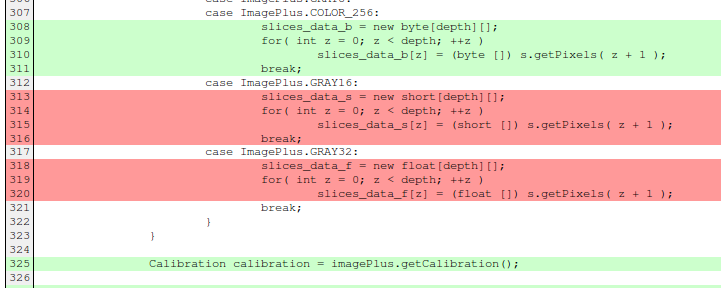
\includegraphics[width=15cm]{bilder/Coverage}
\caption{Couverture du code exemplaire} \cite{codecoverage}
\label{fig:coverage}
\end{figure}


\subsection{Information en retour continue}

Pendant le processus de construction il est indispensable de savoir ce qui se passe. Chaque étape de construction doit fournir des informations à tous les personnes affecté. Classiquement c'est réalisé par envoyer un courriel aux personnes clés. Les possibilités plus modernes sont des plugins et notifications directement dans l'environnement de développement(Team Explorer for TFS intégré dans Visual Studio), dans une application de online-chat (TravisCI native, TeamCity, Jenkins avec plugins), comme message sur l'ordiphone ou dans le système d'exploitation (Native dans Windows 10 ou avec différents applications tierce partie).

\newpage
\subsection{Déploiement continue}

Le déploiement continue est un moyen pour délivrer la version actuelle d'une application aux utilisateurs immédiatement. Si un développeur fait un changement, la construction est initié automatiquement. Après ça les testes unitaires sont exécuté. Si tout les tests complète avec succès  le développeur est informé et l'exécution des testes d'acceptation automatisées commence. Si la fonctionnalité du logiciel est assuré une nouvelle version est déployé immédiatement.
Il est très probable que ce processus est différent dans une autre entreprise ou applications. Les testes d'utilisateur ou des autre contrôles manuelles pourrait être exiger.\\
\begin{figure}[H]
\centering
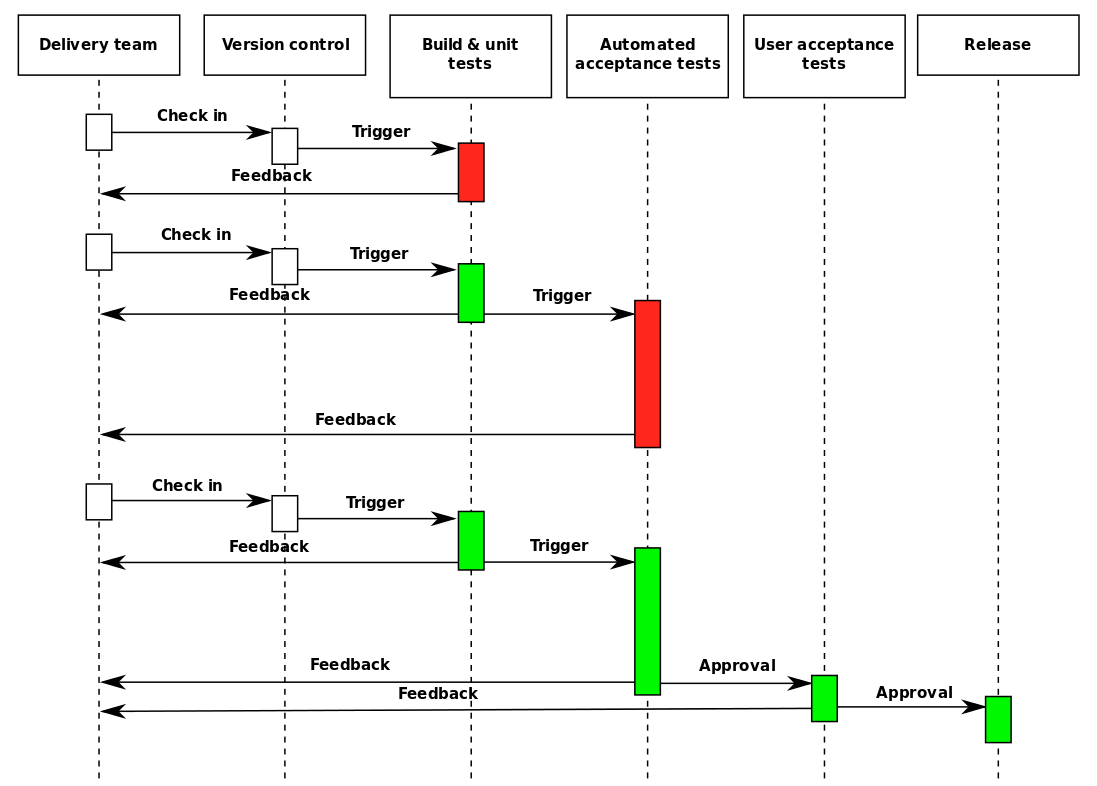
\includegraphics[width=15cm]{bilder/Continuous_Delivery}
\caption{Graphique déploiement continue}\cite{wikicd}
\label{fig:continousdelivery}
\end{figure}

Un autre scénario très fréquent est qu'on a plusieurs environnements et serveurs pour déployer une application (local, development, testing, production). Un déploiement sur la plateforme development seras moins critiques qu'un déploiement sur la production.

\begin{figure}[H]
\centering
\includegraphics[width=15cm]{bilder/Deployment_ci}
\caption{Déploiement continue - Environnements}\cite{bizagigraphique}
\label{fig:continousdelivery}
\end{figure}
\chapter{Évaluation}
\label{eval}

\section{Logiciels de construction}
Pour tester les logiciels de construction nous avons compilé des projets de test de différent largeur sur les systèmes mesurant le temps.
\subsection{Ant}
\begin{tabular}{l|c}
	Largeur&Temps(secondes)\\
		Petit1&7.54\\
		Petit2&8.01\\
		Petit3&7.57\\
		Grand1&27.42\\
		Grand2&35.25\\
		Grand3&28.17\\
\end{tabular}
\subsection{Maven}
\begin{tabular}{l|c}
	Largeur&Temps(secondes)\\
	Petit1&6.56\\
	Petit2&7.10\\
	Petit3&6.49\\
	Grand1&24.32\\
	Grand2&23.45\\
	Grand3&25.01\\
\end{tabular}
\subsection{Gradle}
\begin{tabular}{l|c}
	Largeur&Temps(secondes)\\
	Petit1&3.26\\
	Petit2&3.37\\
	Petit3&3.41\\
	Grand1&11.43\\
	Grand2&12.25\\
	Grand3&12.05\\
\end{tabular}

\subsubsection{Conclusion}
Gradle a des resultats meilleur que Ant et Maven, mais c'est plus compliqué a apprendre. Aussi la documentation de gradle n'est pas tres facile a comprendre parce-que elle est trops détaillé.
\newpage
\section{Serveur de l'intégration continue}

\subsection{Definition des critères}

En dessous vous trouvez les critères avec une bref déscription qui seront utilisé pour evaluer les quatres serveurs de l'intégration continue qui ont été choisit pour ce travail. \footnote{\cite{ibmciserver}}

\begin{enumerate}
\item \textbf{Caractéristiques du produit} \\
\textit{Les charactéristiques du produit sont l'aspect le plus important quand on choisit un serveur d'IC. On doit savoir les éxigences qu'une entreprise a et de ce point de vue selectionner un logiciel.}
	\begin{itemize}
		\item Intégration avec des outils de gestion des versions \\
		\textit{Est l'outil que nous utilisons supporté? Quelles outils sont supporté?}
		\item Intégration avec l'outil de construction \\
		\textit{Est notre langage de programmation (compilateur) et notre outil de construction supporté?}
		\item Information en retour \\
		\textit{Quelles méthodes de l'information en retour existe et sont ils suffisant pour nous?}
		\item Labeling \\
		\textit{Est-il possible de donner des identifiers à des versions d'un logiciel?}
		\item Extensibilité \\
		\textit{Est-il possible d'écrire des extension propre pour le serveur si necessaire?}
	\end{itemize}
\item \textbf{Générale}
	\begin{itemize}
		\item Fiabilité et longévité
		\item Environnement cible
		\item Infrastructure
		\item Couts
		\item Type de logiciel
	\end{itemize}
\item \textbf{Taille de la communauté}
	\begin{itemize}
		\item Nombre d'utilisateurs
		\item Nombre de plug-ins
	\end{itemize}
\item \textbf{Utilisation}
	\begin{itemize}
		\item Facilité d'utilisation
		\item Complexité de l'installation
	\end{itemize}
\end{enumerate}
\newpage
\begin{landscape}
\subsection{Apercu des resultats}
\begin{table}[H]
	\centering
		\begin{tabular}{lp{4cm}p{4cm}p{4cm}p{4cm}} \toprule
			\textbf{Critères} & \href{https://jenkins-ci.org}{\textbf{Jenkins}} & \href{https://www.jetbrains.com/teamcity/}{\textbf{TeamCity}} & \href{https://travis-ci.org}{\textbf{Travis CI}} & \href{https://www.visualstudio.com/en-us/products/tfs-overview-vs.aspx}{\textbf{Team Foundation Server}} \\ \midrule
			\rowcolor{GrayRow}\textbf{Caractéristique du produit} &  &  &  &  \\ \midrule[0.16em]
			Outils de gestion des versions & Subversion/CVS(+plugins) & Subversion/CVS(+plugins) & github/Git & Git/TFVC \\ \midrule
			Outils de construction & & ++ (CLI) & + & \\ \midrule
			Information en retour & & + & ++ & \\ \midrule
			Labeling & & \checkmark & x & \\ \midrule
			Extensibilité & ++ & + & - & -- \\ \midrule
			\rowcolor{GrayRow}\textbf{Générale} &  &  &  &  \\ \midrule[0.16em]
			Fiabilité et longévité & \checkmark & \checkmark & \checkmark & \checkmark \\ \midrule
			Environnement cible & tous & tous & Linux & Microsoft Windows \\ \midrule
			Infrastructure & On-premises & On-premises & On-premises/SaaS & On-premises/SaaS \\ \midrule
			Couts & gratuit & Freemium* & Freemium* & Freemium \\ \midrule
			Type de logiciel & Open Source (MIT) & Propriétaire & Open Source (MIT) & Propriétaire \\ \midrule
			\rowcolor{GrayRow}\textbf{Taille de la communauté} & & & & \\ \midrule[0.16em]
			Nombre d'utilisateurs & many & 30'000 clients & 240'000 projets & many \\ \midrule
			Nombre de plugins & ++ & + & x & - \\ \midrule
			\rowcolor{GrayRow}\textbf{Utilisation} &  &  &  &  \\ \midrule[0.16em]
			Facilité d'utilisation & many & + & ++ & many \\ \midrule
			Complexité de l'installation & many & + & ++ & many \\
			\bottomrule[0.16em]
		\end{tabular}
	\caption{Serveurs de l'IC}
	\label{tab:serveurs_eval}
\end{table}
Freemium = C'est gratuit pour la version base, mais ca coute pour des editions plus grande (entreprise).\\
* free for open source projects
\footnote{\citep{jenkinsplugins} \citep{teamcityenv} \citep{tfsversioncontrol}}

\end{landscape}
\newpage




\subsection{Jenkins}
\begin{wrapfigure}{r}{0.2\textwidth}
  \begin{center}
    
\includegraphics[width=0.18\textwidth]{bilder/JENKINS}
  \end{center}
  \caption{Jenkins Logo}
\end{wrapfigure}
\paragraph{Characteristique du produit} Bien que Jenkins est écrit en Java il est capable de construire beaucoup des langues différents (PHP, Ruby, .Net avec des plugins et tout les autres lancent un script batch ou shellscript dépendent au système d'exploitation). Il y a une nouvelle version de Jenkins chaque semaine (utilisant IC avec soi-même trouvé sur https://www.jenkins-ci.org/).

\paragraph{Générale} Jenkins est un fork de l'outil Hudson qui était développe par Kohsuke Kawaguchi chez Sun Microsystems en 2008. Deux ans plus tardes Kohsuke a eu des différences avec son nouveau employeur Oracle. Il a quité et en 2011 présente la première version de Jenkins. Jenkins est un logiciel code source ouvert écrit en Java licenciée MIT. 
\paragraph{Taille de la communauté} Aujourd'hui Jenkins est installé sur 127000 machines\footnote{\citep{jenkinsstats}}. Sur la site web officielle de Jenkins il y a des plug-ins à toutes fins.(1000++) 
\paragraph{Utilisation} Âpres lancer le service de Jenkins on peut ouvrir l' interface web sur 127.0.0.1:8080. Là on peut definer des build-jobs, gérer les droits d'accès, changer des paramètres et plus. Au début le systeme gestion de version Git n'est pas inclue, seulement CVS et SVN mais il y a un plugin. L'interface d'administration est très facile à utiliser.
\begin{figure}[H]
	\centering
		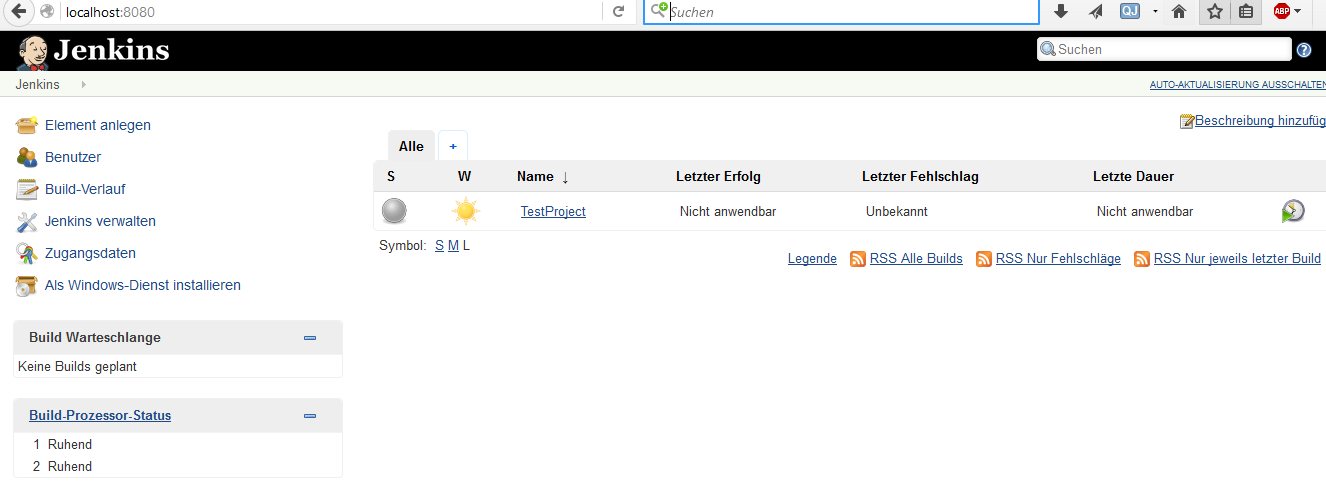
\includegraphics[width=15cm]{bilder/JenkinsGui}
	\caption{Jenkins intérface d'administration}
	\label{fig:jenkinsgui}
\end{figure}













\clearpage
\subsection{TeamCity}
\begin{wrapfigure}{r}{0.2\textwidth}
  \begin{center}
    
\includegraphics[width=0.18\textwidth]{bilder/teamcity512}
  \end{center}
  \caption{TeamCity Logo}
\end{wrapfigure}
\paragraph{Characteristique du produit} TeamCity est un serveur de l'intégration continue de JetBrains, les fabricants d'une grande nombre d'outil de developpment (comme IntelliJ). Il est optimisé pour construire des projets de Java ou .NET, mais supporte aussi Python, Ruby et beaucoup d'autre langage avec des plugins. De plus il existe l'option de travailler avec la ligne de commande. TeamCity est très adaptable et peut être individualiser extensivement. \\
Tous les configurations et tous l'utilisation est effectué par l'interface web. Comme voies d'information en retour TeamCity supporte des émails, des messages Jabber ou directement dans l'IDE. De plus TeamCity supporte des "Build Tag" pour identifier des constructions. Si la functionalité de TeamCity ne suffice pas, il est facilement possible d'écrire un plugin.

\paragraph{Générale} L'infrastructure pour soutenir TeamCity doit être mis en place par l'entreprise. Il existe trois options de licence de TeamCity.
\begin{itemize}
	\item TeamCity Professional (20 configurations et 3 agent de construction)
	\item TeamCity Enterprise (3-100 agent packs)
	\item TeamCity Additional Build Agent (+ 1 agent de construction)
\end{itemize}
La licence TeamCity Professional est gratuite mais limité. Pour les versions TeamCity Enterprise le nombre de projets est illimité, mais on peu incrementer le nombre d'agent de construction pour atteindre une meilleure pérformance quand il y a beaucoup de processus de construction en même temps. Pour des projéts Open Source TeamCity est gratuite, pour des jeunes pousses il y a des rabais.\footnote{\citep{teamcitybuy}}
\paragraph{Taille de la communauté}
JetBrains affirme que 30'000+ clients utilise TeamCity pour executer l'intégration continue (Boeing, HP...). Il y a une grande nombre de plugins disponible sur le page web de TeamCity.\footnote{\citep{teamcityplugins}}
\paragraph{Utilisation}
L'installation de TeamCity est assez facile. Il existe des archive des fichiers exprès pour des installations rapide. TeamCity est basé sur Java et utilise un serveur Tomcat. Pour l'installation rapide, tous ce qu'on devait faire est télécharger et extraire l'archive, et puis executer un script et completer la configuration intiale. Pour un système productive une installation un peu plus complexe est prévu.\\
En utilisant TeamCity en premier on est confondu par la grande nombre d'options de configuration. Mais quand-même il était possible et pas très difficile de construire et mettre en rapport notre environment teste. TeamCity est très volumineux, mais bien structuré et agréable pour l'utilisateur. Le faite qu'on peut faire toute la configuration sur l'interface web est un grande plus.
\begin{figure}[H]
	\centering
		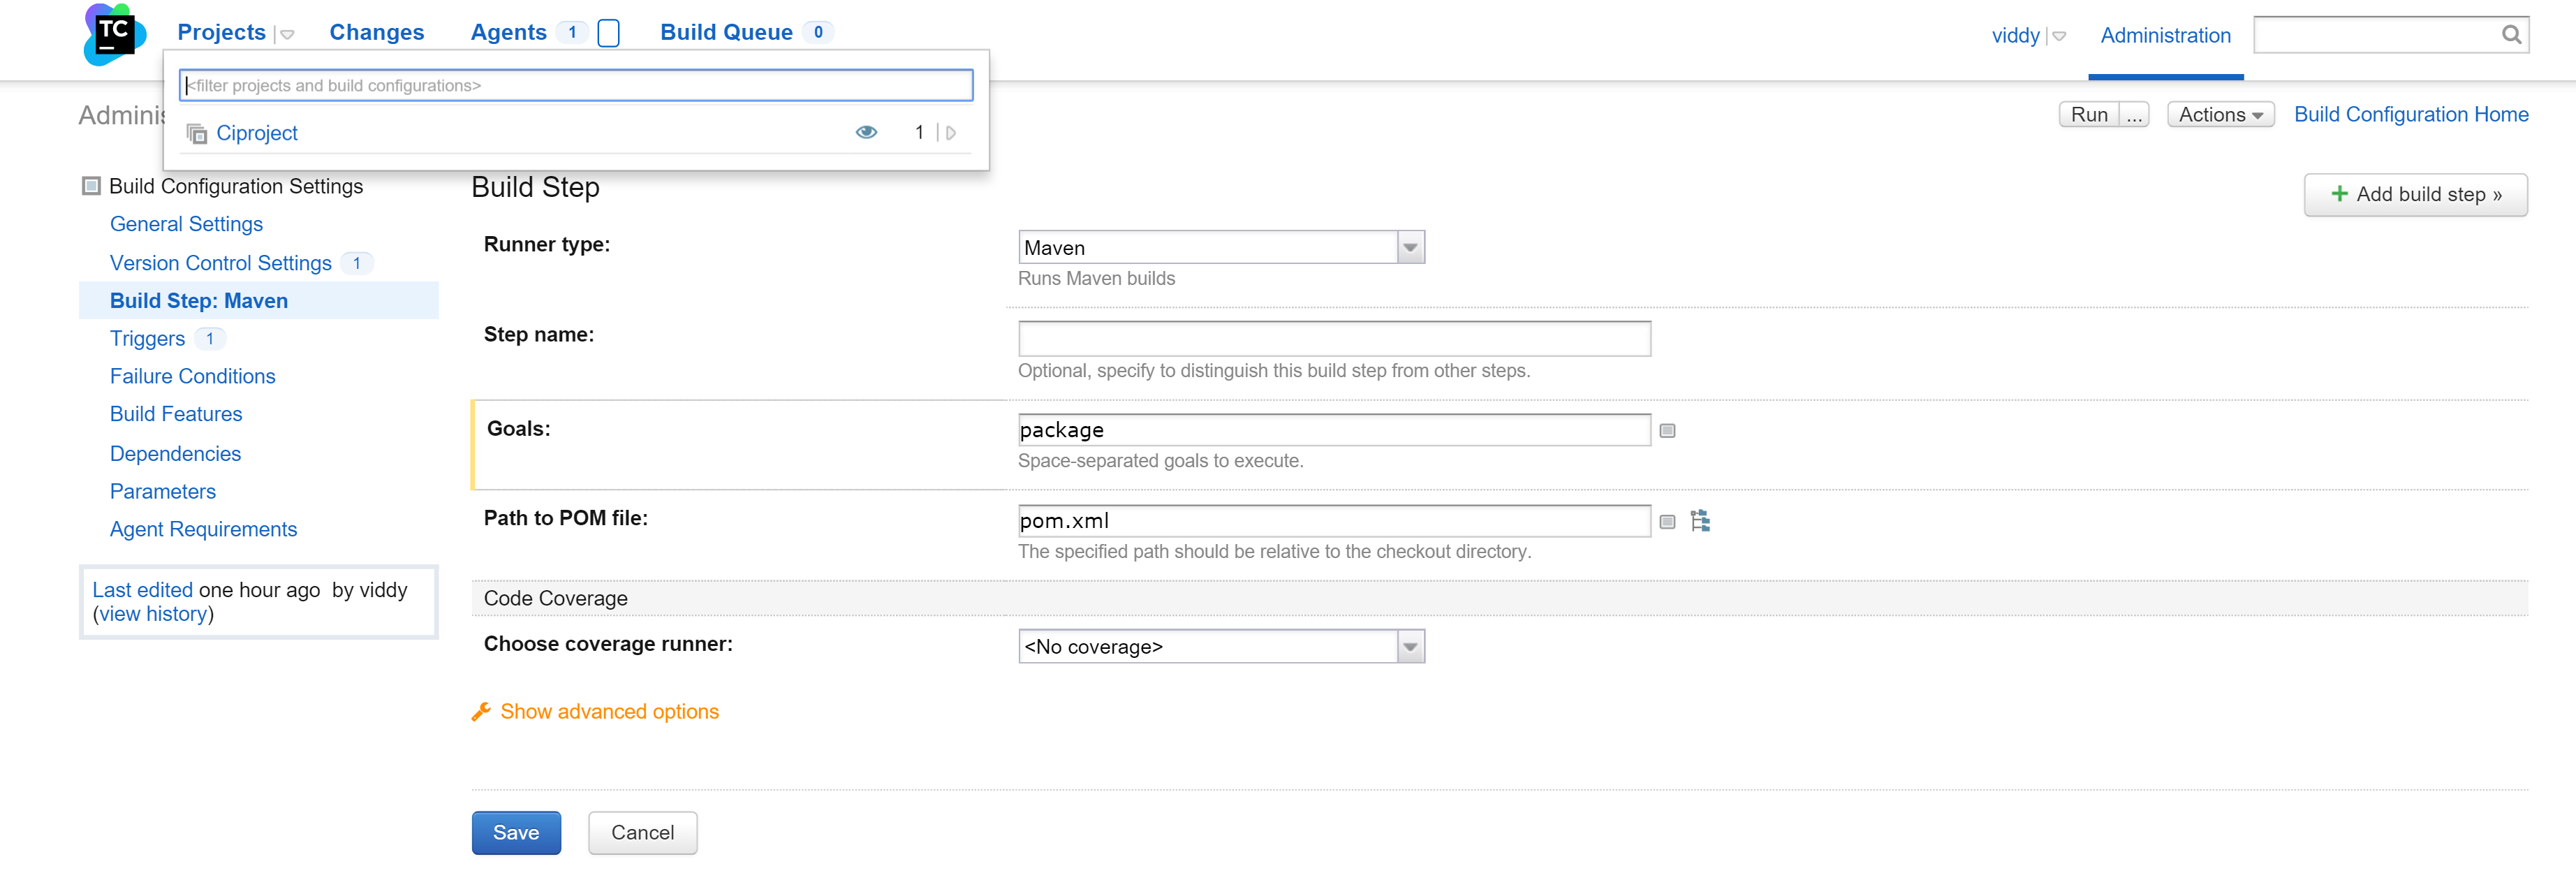
\includegraphics[scale=0.35]{bilder/teamcityadmin}
	\caption{TeamCity intérface d'administration}
	\label{fig:travisgui}
\end{figure}





\clearpage
\subsection{Travis CI}
\begin{wrapfigure}{r}{0.4\textwidth}
  \begin{center}
    
\includegraphics[width=0.38\textwidth]{bilder/Travis-CI-logo}
  \end{center}
  \caption{Travis CI Logo}
\end{wrapfigure}
\paragraph{Characteristique du produit}
Travis CI est un serveur de l'intégration continue très facile à mettre en service et avec une intégration excellente avec \href{https://github.com/}{github.com}. Il supporte beaucoup de différent langage et outil de construction. La liste complète peuvent être trouver dans la documentation\footnote{\citep{traviscidocs}}. Mais il seulement supporte git comme outil de gestion des versions.\\
De plus il offre multiple voies d'information en retour. Le plus facile est par email, mais il y a aussi la possibilité d'envoyer des messages par IRC, Slack, HipChat etc.\footnote{\citep{traviscinotification}}. Chaque construction recoit un identificateur numerique, mais il n'est pas possible de le changer. Il y a une API pour accéder à Travis (SaaS), mais l'extensibilité semble limité.

\paragraph{Générale}
Il existe trois version de Travis CI.
\begin{itemize}
	\item \href{https://travis-ci.org/}{Travis CI for Open Source}
	\item \href{https://travis-ci.com/}{Travis Pro}
	\item \href{https://enterprise.travis-ci.com/}{Travis Enterprise}
\end{itemize}
Les deux première versions sont accessible comme SaaS. Une version est pour des projets Open Source qui est gratuite et l'autre est pour des projets avec un dépot de github privée qui coute. La troisième version est pour des entreprises qui veulent mettre l'infrastructure comme des serveurs à disposition eux-mêmes (Linux).

\paragraph{Taille de la communauté}
Travis CI affirme sur la page web qu'il y a 246'506 projets Open Source qui sont testé et intégré sur leur platform. Sur la nombre d'utilisateurs des deux versions commercial il n'y a pas d'information.

\paragraph{Utilisation}
L'utilisation de Travis CI est très pratiques est facile. Si on a déja un dépot sur github, il faut seulement trois pas pour lancer l'intégration continue avec Travis.

\begin{enumerate}
	\item Login avec le compte de github sur travis
	\item Choisir le dépot
	\item Écrire un fichier .travis.yml pour définir la configuration
\end{enumerate}

Après ça chaque fois qu'il y a un changement sur le dépot les testes et la construction seras executé automatiquement. Pour construire notre projet de test en java (maven), d'executer les testes avec trois différent version de java et envoyer un email à une adresse si quelque chose ne marche pas, le fichier en bas suffisait. De plus vous trouver un apercu de l'interface d'administration de travis.

\begin{figure}[H]
	\centering
		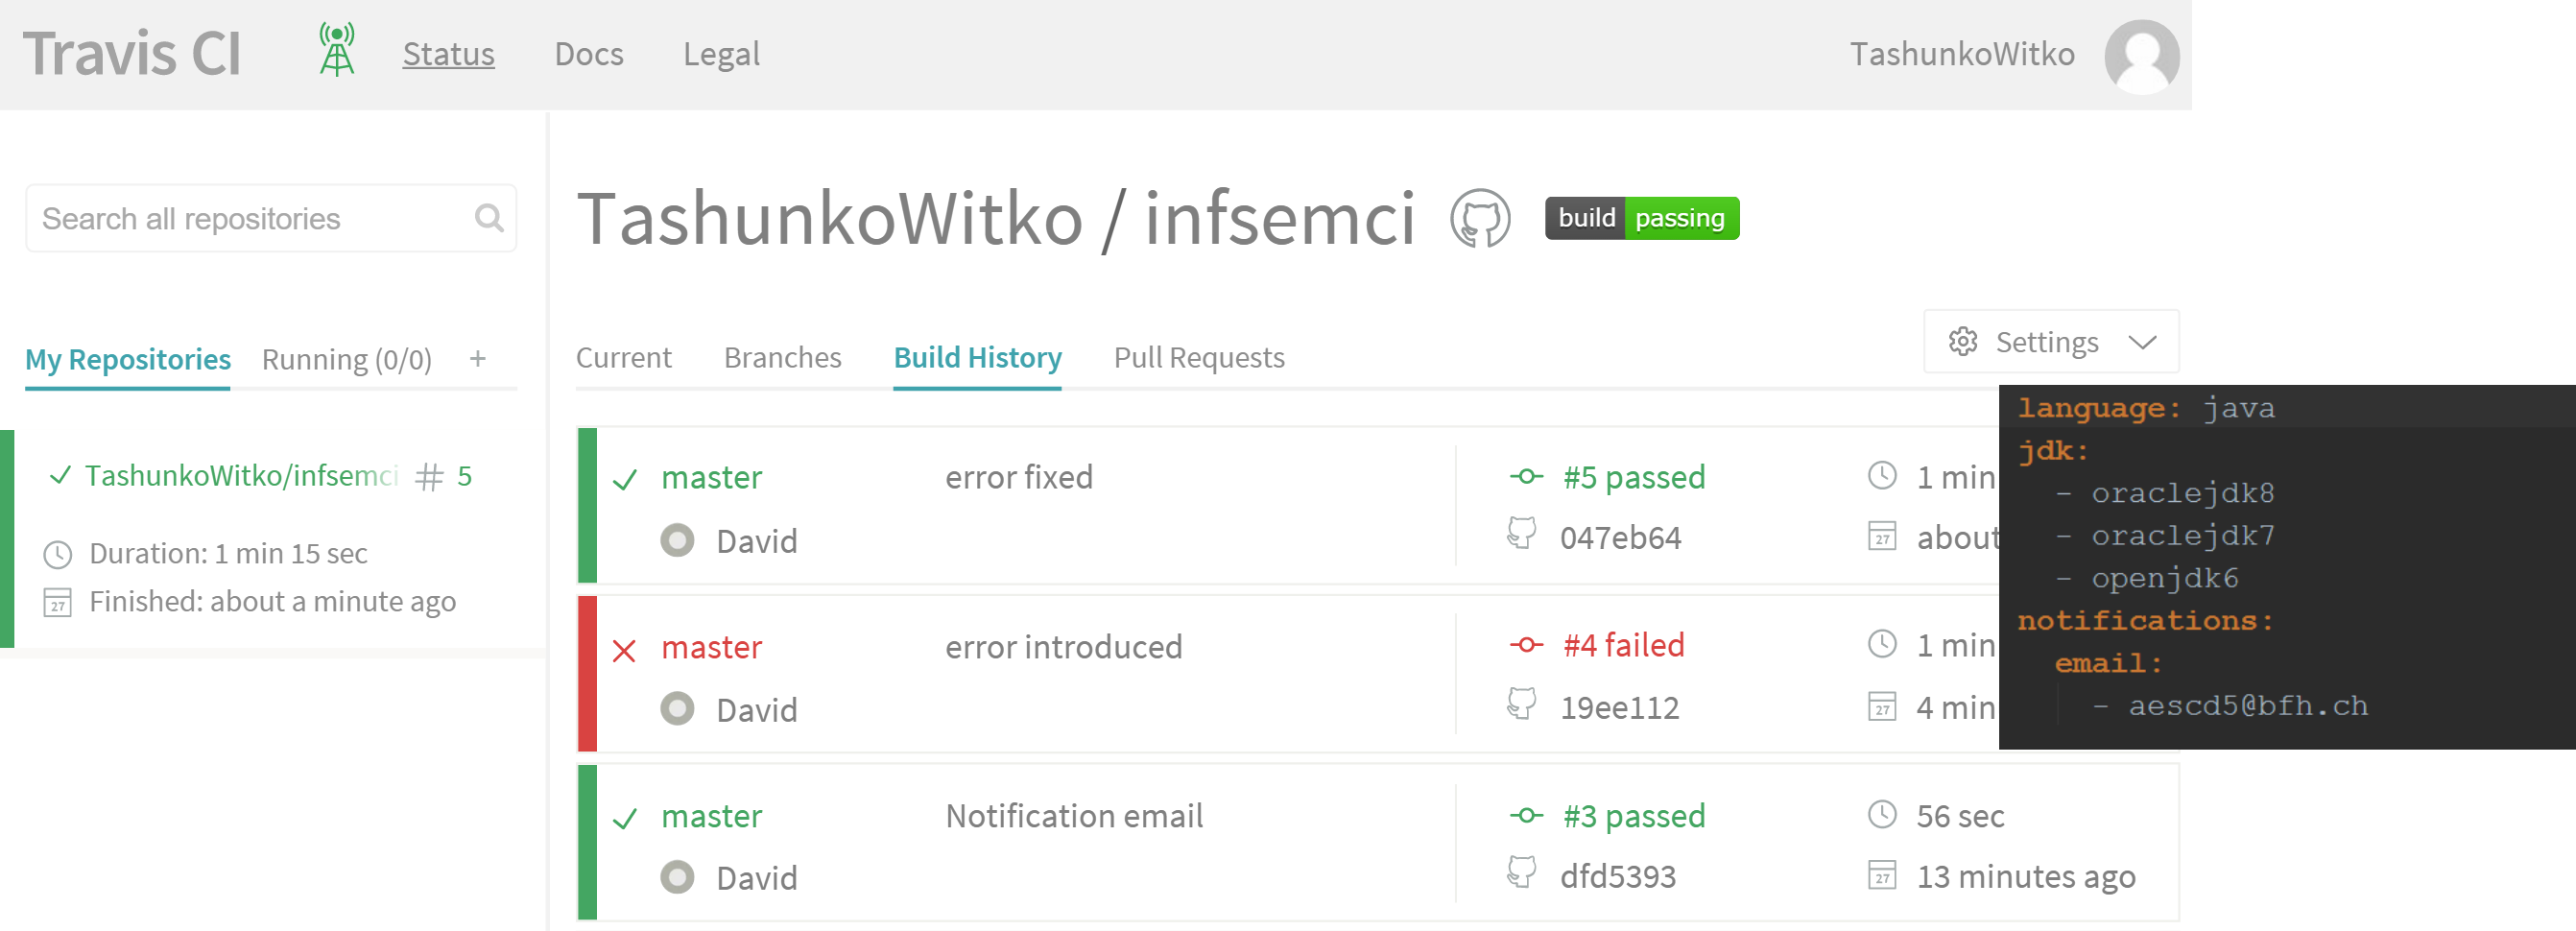
\includegraphics[scale=0.2]{bilder/travisciymlfile}
	\caption{Travis intérface d'administration et yml fichier}
	\label{fig:travisgui}
\end{figure}





\clearpage
\subsection{Team Foundation Server}
\paragraph{Characteristique du produit} TFS est la forge logicielle de Microsoft. Le cycle de vie entier du logiciel agile est couvert. La gestion des versions(TFVC ou Git), des builds, des résultats de test et beaucoup plus depuis on peut installer des plug-in gratuit et payée facilement. Il y a une version "On-premises" qui est installé sur une machine/un serveur de l'entreprise mise a jour une fou par trimestre par Windows Update Services. Si on veut avoir la version la plus actuelle à n'importe quel temps il y a un service en ligne, fourni par Microsoft sur la nuage Azure.

\paragraph{Générale}  Le prix pour la version "On-premises" est calculé le même que pour la version SaaS listé en bas.
\begin{itemize}
\item[<5 personnes] Gratuit, Temps de construction inclue 240 minutes/mois
\item[6-10 personnes] CHF 5.40/personne et mois
\item[11-100 personnes]  CHF 7.20/personne et mois
\item[101-1000 personnes]  CHF 3.60/personne et mois
\item[>1001 personnes]  CHF 1.80/personne et mois
\item[Agent de construction additionnel (hosted)]  CHF 36.10/agent
\item[Agent de construction additionnel (locale)]  CHF 13.50/agent
\end{itemize}
Combiné avec une suscription MSDN beaucoup des services VisualStudio et Azure sont inclue.
\paragraph{Taille de la communauté} Sur le nouveau magasin en ligne on peut télécharger nombreux plug-ins publié par Microsoft ou des développeurs indépendantes. Il y a des addons pour Visual Studio, VisualStudioCode et VisualStudio TeamServices gratuit et payé.
\paragraph{Utilisation} L'interface utilisateur es très intuitive. Apres la registration on peut lié un projet locale avec le projet team en ligne. Si on veut configurer la construction ou le déploiement automatisé il faut ouvrir l'interface web et suivre les instructions. 
la partie test est un peu confus au debut, parce que les tests unitaires et les tests d'integration sont inclue dans la construction et dans le chapitre test sont les tests d'acceptation recordé.

\begin{figure}[H]
	\centering
		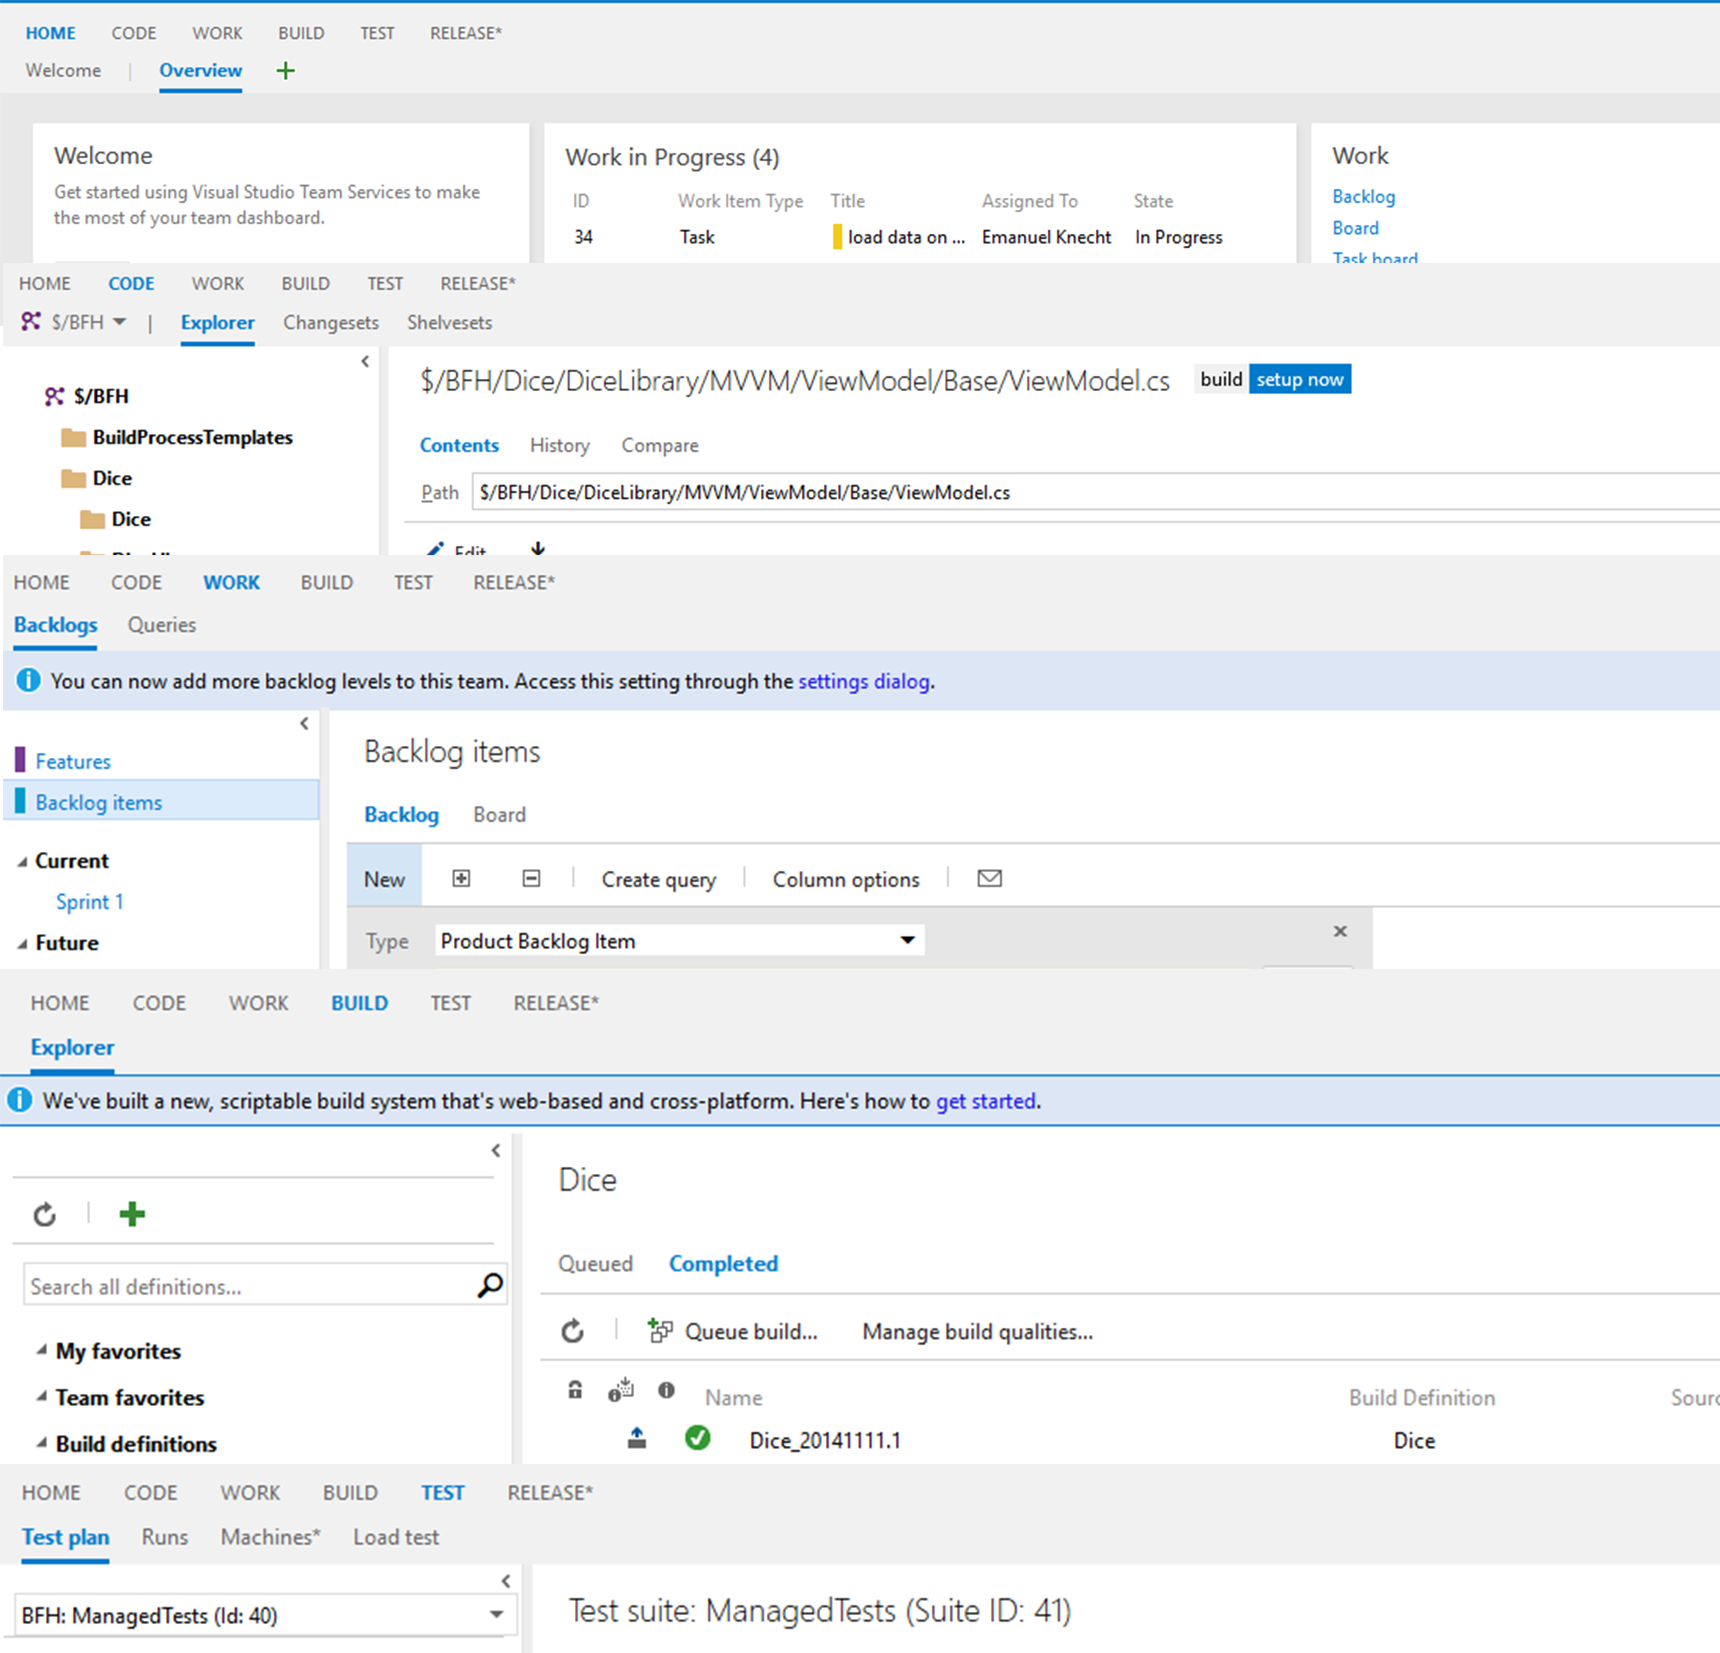
\includegraphics[height=10cm]{bilder/vso}
	\caption{Visualstudio Online interface d'administration}
	\label{fig:vsogui}
\end{figure}


\chapter{Conclusion}
\label{chap:conclusion}

\section{Bilan}

%---------------------------------------------------------------------------

% Selbständigkeitserklärung
%---------------------------------------------------------------------------
%\cleardoublepage
%\phantomsection 
%\addcontentsline{toc}{chapter}{Selbständigkeitserklärung}
%\chapter*{Selbst�ndigkeitserkl�rung}
\label{chap:selbstaendigkeitserklaerung}

\vspace*{10mm} 

Ich/wir best�tige/n, dass ich/wir die vorliegende Arbeit selbstst�ndig und ohne Benutzung anderer als der im Literaturverzeichnis angegebenen Quellen und Hilfsmittel angefertigt habe/n. S�mtliche Textstellen, die nicht von mir/uns stammen, sind als Zitate gekennzeichnet und mit dem genauen Hinweis auf ihre Herkunft versehen. 

\vspace{15mm}

\begin{tabbing}
xxxxxxxxxxxxxxxxxxxxxxxxx\=xxxxxxxxxxxxxxxxxxxxxxxxxxxxxx\=xxxxxxxxxxxxxxxxxxxxxxxxxxxxxx\kill
Ort, Datum:		\> [Biel/Burgdorf], \versiondate \\ \\ 
Namen Vornamen:	\> [Test Peter] 	\> [M�ster R�s�] \\ \\ \\ \\ 
Unterschriften:	\> ......................................\> ...................................... \\
\end{tabbing}

%---------------------------------------------------------------------------

% Glossary
%---------------------------------------------------------------------------
%%\cleardoublepage
%\phantomsection 
%\addcontentsline{toc}{chapter}{Glossar}
%\renewcommand{\glossaryname}{Glossar}
%\printglossary
%---------------------------------------------------------------------------

% Bibliography
%---------------------------------------------------------------------------
\phantomsection 
\addcontentsline{toc}{chapter}{Bibliographie}
\bibliographystyle{IEEEtranS}
\bibliography{datenbanken/bibliography}{}
%---------------------------------------------------------------------------

% Listings
%---------------------------------------------------------------------------
\phantomsection 
\addcontentsline{toc}{chapter}{Table des figures}
\listoffigures
\phantomsection 
%\addcontentsline{toc}{chapter}{Tabellenverzeichnis}
%\listoftables
%---------------------------------------------------------------------------

% Attachment:
%---------------------------------------------------------------------------
\appendix
\settocdepth{section}
%---------------------------------------------------------------------------

%---------------------------------------------------------------------------
\end{document}

